\documentclass{article}
\usepackage[T1,T2A]{fontenc}
\usepackage[utf8]{inputenc}
\usepackage[english,russian]{babel}

\usepackage[left=3cm,right=3cm,
    top=3cm,bottom=3cm,bindingoffset=0cm]{geometry}

\usepackage{graphicx}
\usepackage{color}
\usepackage{hyperref}
\usepackage{amsmath}
\usepackage{amsfonts}
\usepackage{amssymb}


\usepackage{setspace}
\usepackage{indentfirst}
\usepackage{textcomp}
\usepackage{ifthen}
\usepackage{calc}
\usepackage{mathrsfs}
\usepackage[dvipsnames]{xcolor}


\title{Введение в машинное обучение}
\author{Национальный исследовательский университет "Высшая школа экономики" \and Yandex School of Data Analysis\\\\
Неофициальный конспект по курсу.}

\begin{document}
\maketitle
\tableofcontents
\newpage

\section{Метрические методы}
\subsection{Определение}
Следующие методы, которые мы рассмотрим, будут \textbf{метрические методы}, которые используют функции \textit{расстояния} или \textit{метрики} в пространстве объектов.

Исходная идея заключается в предположении, что в практических задачах часто встречаются зависимости, которые непрерывны (хотя это справедливо скорее для задач регрессии, уточнения описаны ниже):

\begin{itemize}
\item \textbf{Гипотеза непрерывности} (для регрессии):

\begin{center}
\textcolor{red}{близким объектам соответствуют близкие объекты.}
\end{center}

\item \textbf{Гипотеза компактности} (для классификации):

\begin{center}
\textcolor{red}{близкие объекты, как правило, лежат в одном классе.}
\end{center}

\end{itemize}

Впрочем, далее в этом документе мы будем рассматривать \textit{метрические методы} именно для \textit{задач классификации}, регрессия будет потом. 

Теперь зададимся вопросом, как формализовать эту <<близость>>?

\begin{itemize}
\item \textbf{Формализация понятия <<близости>>:}

\qquad Задана функция расстояния $\rho : X \times X \rightarrow [0, \infty)$.
\end{itemize}

По сути эта функция от пары объектов, которая паре ставит соответствие --- неотрицательное число.

Часто также накладывают требование, чтобы это была метрика в пространстве объектов, то есть чтобы она была и симметричной, и выполнялось неравенство треугольника. Однако формально в методах нигде не используется предположение о том, что это метрика, поэтому, в общем-то, и функции расстояния, не являющиеся метриками, нам тоже подходят.

\subsection{Примеры расстояний в задачах}
\subsubsection{Евклидово пространство и его обобщение}

Самым известным примером расстояния, наверное, является \textbf{евклидово расстояние} в признаковом пространстве. Также ее эту конструкцию можно обобщить (добавить иную степень, или ввести веса признаков), и мы получим два следующих варианта:

$$\rho(x, x_i) = \Biggr(\sum\limits_{j = 1}^n |x^j - x_i^j|^2\Biggl)^\frac{1}{2}
\qquad\qquad\qquad
\rho(x, x_i) = \Biggr(\textcolor{red}{w_j}
\sum\limits_{j = 1}^n |x^j - x_i^j|^{\textcolor{red}{p}}
\Biggl)^{\textcolor{red}{\frac{1}{p}}}$$

$x = (x^1, \ldots, x^n)$ --- вектор признаков объекта $x$.

$x_i = (x_i^1, \ldots, x_i^n)$ --- вектор признаков объекта $x_i$.
\\

Впрочем, обобщенный вариант требует дополнительных усилий, неких процедур, которые будут обучать эти дополнительные параметры.

\subsubsection{Редакторское расстояние Левенштейна}

Далеко не всегда, не во всех задачах, именно использование евклидовой метрики осмысленно, и есть масса задач, где у нас исходно \textit{нет признаковых описаний объектов}, и гораздо проще пользоваться не признаками, а \textit{непосредственно} мерять расстояние между объектами. 

Примеры таких объектов --- это \textit{символьные строки}. Это могут быть тексты естественного языка, это могут быть нуклеотидные или аминокислотные последовательности, которые изучаются в биоинформатике. 
\\

В таких задачах, чтобы сравнить текстовые строки, вообще говоря, произвольной длины, часто используется так называемое \textbf{редакторское расстояние Левенштейна} --- это количество вставок и замен символов, которое необходимо произвести, чтобы привести одну строку в другую:

\begin{center}

CTGGG\textcolor{green}{GTA}AAA\textcolor{red}{GGTC}CCTTAGCC....TTTA\textcolor{green}{G}AAAAA..GGGCCATTAGG\textcolor{red}{AAA}TTGC

CTGGG\textcolor{green}{ACT}AAA..........CCTTAGCC\textcolor{red}{TA}TTTA\textcolor{green}{C}AAAAA\textcolor{red}{T}GGGCCATTAGG........TTGC
\end{center}

Описать две сравниваемых строки признаками было бы намного труднее, чем посчитать подобное расстояние, которое к тому же достаточно эффективно считается.

\subsubsection{Энергия сжатий и растяжений}

Следующий пример уже между объектами еще \textit{более сложной природы}: допустим, мы хотим сравнить 2 подписи, которые сделали люди специальным пером электронным, которое запоминает координаты кончика пера ну и еще азимут движения пера. Значит, мы как подпись имеем 3 кривые, 3 временных ряда, и нам нужно сравнивать такие временные ряды:

\begin{center}
    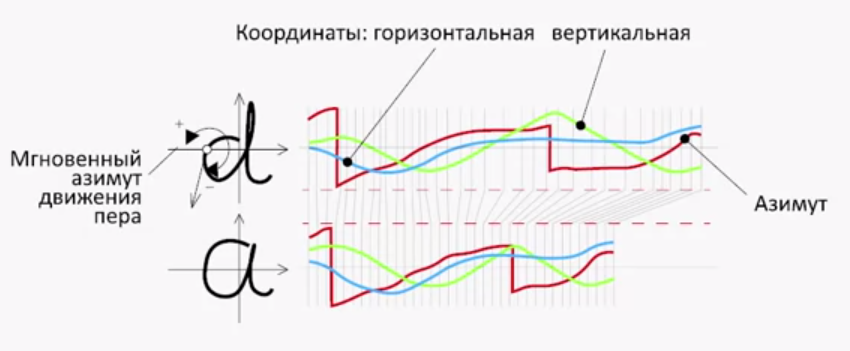
\includegraphics[scale=0.53]{images/4_1.png}
\end{center}

На картинке представлен пример такого сравнения, когда 2 похожие буквы сравниваются, и мы видим, что эти 3 кривые они очень \textit{похожи} с точностью до каких-то \textit{сжатий, растяжений, выравниваний}.

Можно придумать модель расстояния между такими траекториями, как \textit{модель пружинок}, которые слегка сжимаются или растягиваются между маленькими локальными кусочками этих кривых, и посчитать энергию сжатий и растяжений пружинок --- это и будет \textit{расстояние} между этими объектами.
\\

Опять же, расстояние посчитать легко, а придумать здесь признаки было бы значительно сложнее. 

\newpage
\subsection{Обобщенный метрический классификатор}

Допустим, что кто-то нам \textit{уже дал} функцию расстояния и теперь перед нами стоит задача --- \textit{научиться классифицировать объекты}.

Самый простой алгоритм классификации вообще из всех алгоритмов, известных в машинном обучении, --- это \textbf{алгоритм ближайшего соседа}. Чтобы классифицировать объект $x$, возьмем все объекты обучающей выборки и найдем среди них ближайший к $x$, и отнесем $x$ к тому же классу, к которому принадлежит этот объект.

Конечно, использовать для классификации только одного ближайшего соседа --- это не очень удачная идея, лучше взять окрестность, учесть несколько ближайших соседей, как-то по ним усреднить. И поэтому возникает такая \textbf{обобщенная идея}: \textit{упорядочим все объекты обучающей выборки по возрастанию расстояний до нашего классифицированного объекта $x$}:

\begin{center}
\line(1,0){400}
\end{center}

\begin{itemize}
\item Для произвольного $x \in X$ отранжируем объекты $x_1, \ldots, x_l$:

$$\rho(x, x^{(1)} \leqslant \rho(x, x^{(2)} \leqslant \ldots \leqslant \rho(x, x^{(l)},$$

$x^{(i)}$ --- $i$-й сосед объекта $x$ среди $x_1, \ldots, x_l$;

$y^{(i)}$ --- ответ на $i$-м соседе объекта $x$.

\end{itemize}

\begin{center}
\line(1,0){400}
\end{center}

 Дополнительно введем \textit{вес} $i$-того соседа или его \textit{ценность, полезность} при классификации объекта $x$. Будем обозначать этот вес $w(i, x)$, то есть это функция от объекта и от порядкового номера соседа.

Соответственно, если мы \textit{усредним} в каждом классе значение этих весов, то мы получим в итоге оценку близости объекта к классу: мы ее обозначаем Г с индексом $y$ от объекта $x$.Индекс $y$ показывает, что такая оценка она относится к определенному классу. \textit{Таким образом получаем}:

\begin{center}
\line(1,0){400}
\end{center}

\begin{itemize}
\item \textbf{Метрический алгоритм классификации:}
$$\textcolor{red}{a(x, X^l) = arg\ \underset{y \in Y}{max}}
\underbrace{
\textcolor{red}{\sum\limits_{i = 1}^l \bigl[y^{(i)} = y\bigr]w(i, x)}}_{\text{Г}_y(x)},$$

$\textcolor{red}{w(i,x)}$ --- вес, \textit{оценка сходства объекта} $x$ с его $i$-м \textit{соседом}. \\Неотрицательная, не возрастающая по i.

Г$_y(x)$ --- \textit{оценка близости объекта} $x$ к \textit{классу} $y$.

\end{itemize}

\begin{center}
\line(1,0){400}
\end{center}

Cамый естественный принцип классификации --- это отнести объект $x$ к тому классу, для которого эта оценка близости максимальна, что мы и делаем выше.
\\

Соответственно, есть масса частных случаев этой общей формы метрического алгоритма классификации.

\subsubsection{Метод $k$ ближайших соседей ($k$ nearest neighbors, kNN)}

\textbf{Метод ближайших} соседей или его частный самый простой случай --- \textbf{метод первого ближайшего соседа}:

\begin{itemize}
\item[] $w(i, x) = [i \leqslant k]$

\item[] $w(i, x) = [i \leqslant 1]$
\end{itemize}

\textbf{Преимущество} этого метода в том, что он очень просто реализуется. Еще говорят, что это \textit{«ленивое»} обучение, потому что, собственно, никакого обучения здесь не происходит --- мы просто запоминаем выборку, а после классификация заключается в поиске ближайших соседей:

\begin{itemize}
\item простота реализации (lazy learning);
\item параметр $k$ можно оптимизировать по критерию скользящего контроля (leave-one-out):

$$\text{LOO}(k, x^l)=\sum\limits_{i = 1}^l\Bigl[a(x_i;\ X^l\backslash\{x_i\},\ k) \not= y_i]\Bigr]\ 
\rightarrow \underset{q}{min}$$

Дело в том, что если мы берем \textit{слишком мало} соседей, то среди них могут оказаться какие-то случайные шумовые выбросы. Если мы берем \textit{слишком много} соседей, то мы построим слишком простой классификатор, который в любой точке пространства по сути будет выдавать одно и то же значение. И где-то \textit{посередине} находится тот классификатор, который действительно будет прилично работать.
\\
\end{itemize}

\textbf{Проблемы:}

\begin{itemize}
\item Неоднозначность классификации Г$_y(x) = $Г$_s(x),\ y\not=s$.

То есть мы можем столкнуться с ситуацией, когда \textit{для двух классов оценки} степени близости объекта к классу \textit{совпадают}, и мы поэтому не понимаем, к какому из этих двух классов отнести наш объект. (Например, $k$ четное и половина соседей относятся к одному классу, вторая половина к другому.)

\item Мы нигде не учитываем сами значения расстояний.

После того как мы отранжировали объекты обучения по возрастанию расстояний, у нас остались только порядковые номера этих объектов. Может возникнуть ситуация, когда мы, например, классифицируем по пяти ближайшим соседям: четыре соседа находятся действительно близко от объекта, а пятый где-то совсем далеко. Конечно, в таком случае его надо было бы учесть с меньшим весом.
\end{itemize}

\quad
\\

\textbf{Пример зависимости LOO от числа соседей}
\\

Пару слов о том, как происходит \textit{оптимизация} параметра числа ближайших соседей и почему \textit{обязательно} надо использовать функционалы, которые сам классифицируемый объект изымает из обучающей выборки.

\begin{center}
    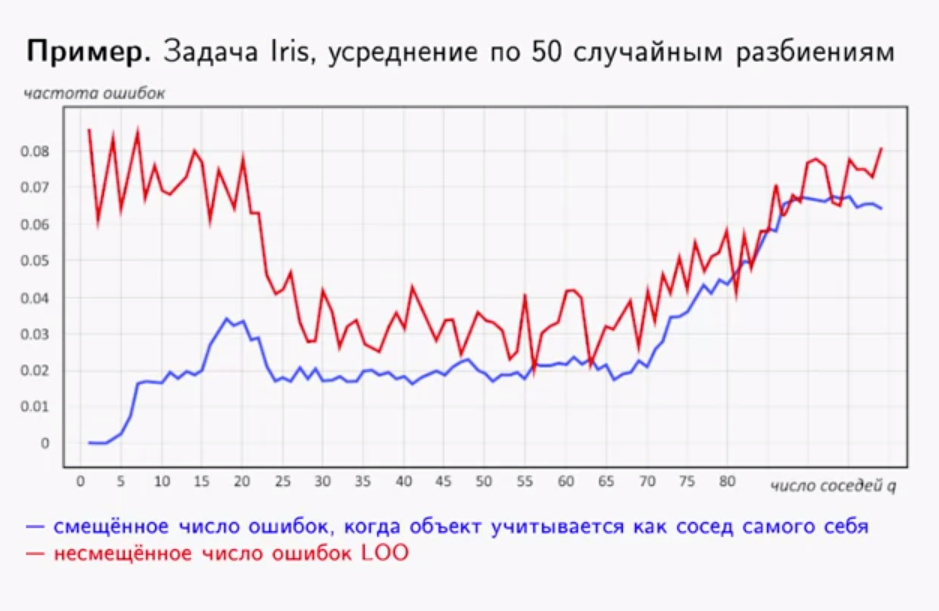
\includegraphics[scale=0.45]{images/4_2.png}
\end{center}

Нам этом графике приведены две кривые: это уже известная нам выборка цветков ириса, и использованы два алгоритма.

Первый алгоритм --- это классификация методом k ближайших соседей. И когда классифицируется некий объект обучающей выборки, сам же он является своим собственным соседом, и это дает синюю кривую. 

Если же сам объект исключается из числа своих соседей, получается красная кривая.
\\

Видно, что синяя кривая нам дает \textit{оптимистически смещенную оценку числа ошибок} на контрольных выборках. Нам кажется, что оптимально использовать одного соседа, но если объект сам же является своим собственным соседом, то понятно, что это некий самообман.

И здесь же на красной кривой мы видим, что в данной задаче оптимально брать где-то от 30 до 60 соседей, а синяя кривая нам дает \textit{ложный} ответ, что надо пользоваться методом первого ближайшего соседа. Этот метод практически никогда не работает надежно.

\newpage
\subsubsection{Метод окна Парзена}

Пойдем дальше и посмотрим, как можно еще обобщить \textit{метод ближайших соседей}, чтобы справиться вот с теми двумя недостатками, которые были отмечены ранее. 
\\

Мы вольны выбирать функцию весов соседей, как мы хотим. Давайте сделаем так, чтобы вес соседа убывал по мере возрастания расстояния до него. 

Введем два новых понятия: это \textbf{ядро} и \textbf{ширина окна}:

\begin{itemize}
\item[] $w(i, x) = K\Bigl(\frac{\rho(x, x^{(i)}}{h}\Bigr)$, где h --- ширина окна,

\item[] $K(r)$ --- ядро, не возрастает и положительно на $[0, 1]$.
\end{itemize}

То есть мы функцию веса зададим как такую конструкцию --- ядро от расстояния поделить на ширину окна ---  и получаем взвешенную функцию, которая \textit{придает меньшие веса тем соседям, которые находятся дальше}.  Этот метод называется \textbf{метод окна Парзера}.

У этого метода есть два варианта:

\begin{center}
\line(1,0){400}
\end{center}

\begin{itemize}
\item Метод парзеновского окна \textit{фиксированной ширины}:

$$A(x;\ X^l, \textcolor{red}{h}, K) = arg\ \underset{y \in Y}{max}
\sum\limits_{i = 1}^l[y_i = y]K\Bigl(\frac{\rho(x, x^{(i)})}{\textcolor{red}{h}}\Bigr)$$

Но это не очень хорошо работает в тех задачах, где плотность распределения объектов неравномерна и есть области пространства, где объекты лежат густо, а в других областях объекты лежат более разреженно, и в таком случае хочется в первой области использовать более узкое окно, а во втором случае --- более широкое.

\item Метод парзеновского окна \textit{переменной ширины}:

$$A(x;\ X^l, \textcolor{red}{k}, K) = arg\ \underset{y \in Y}{max}
\sum\limits_{i = 1}^l[y_i = y]K\Bigl(\frac{\rho(x, x^{(i)})}
{\textcolor{red}{\rho(x, x^{k + 1})}}
\Bigr)$$

Решает предыдущую проблему, и в таком случае в качестве ширины окна берется расстояние до (k + 1) соседа. Это означает, что \textit{для k-ближайших соседей будут ненулевые веса}. И таким образом решается эта проблема неравномерности распределения объектов в пространстве.

\end{itemize}

\begin{center}
\line(1,0){400}
\end{center}


\textbf{Оптимизация параметров} может происходить по тому же критерию LOO:
\begin{itemize}
\item выбор ширины окна $h$ или числа соседей $k$

\item выбор ядра $K$ при этом \textit{слабо влияет} на качество классификации
\\
\end{itemize}

\begin{center}
\line(1,0){400}
\end{center}


\textbf{Пример задачи с парзеновским окном фиксированной ширины $h$}

Пусть у нас есть синтетическая двумерная выборка, объекты в которой принадлежат к двум классам $Y = \{-1, +1\}$.

$$a(x) = arg\ \underset{y \in Y}{max}\text{Г}_y(x)
= sign(\text{Г}_{+1}(x) - \text{Г}_{-1}(x))$$

То есть мы нашу функцию метрического классификатора записали как разность оценка близости объекта $x$ к $(+1)$ классу и оценки близости к $(-1)$ классу. Соответственно, на графике мы это изобразим разными цветами:

\begin{center}
    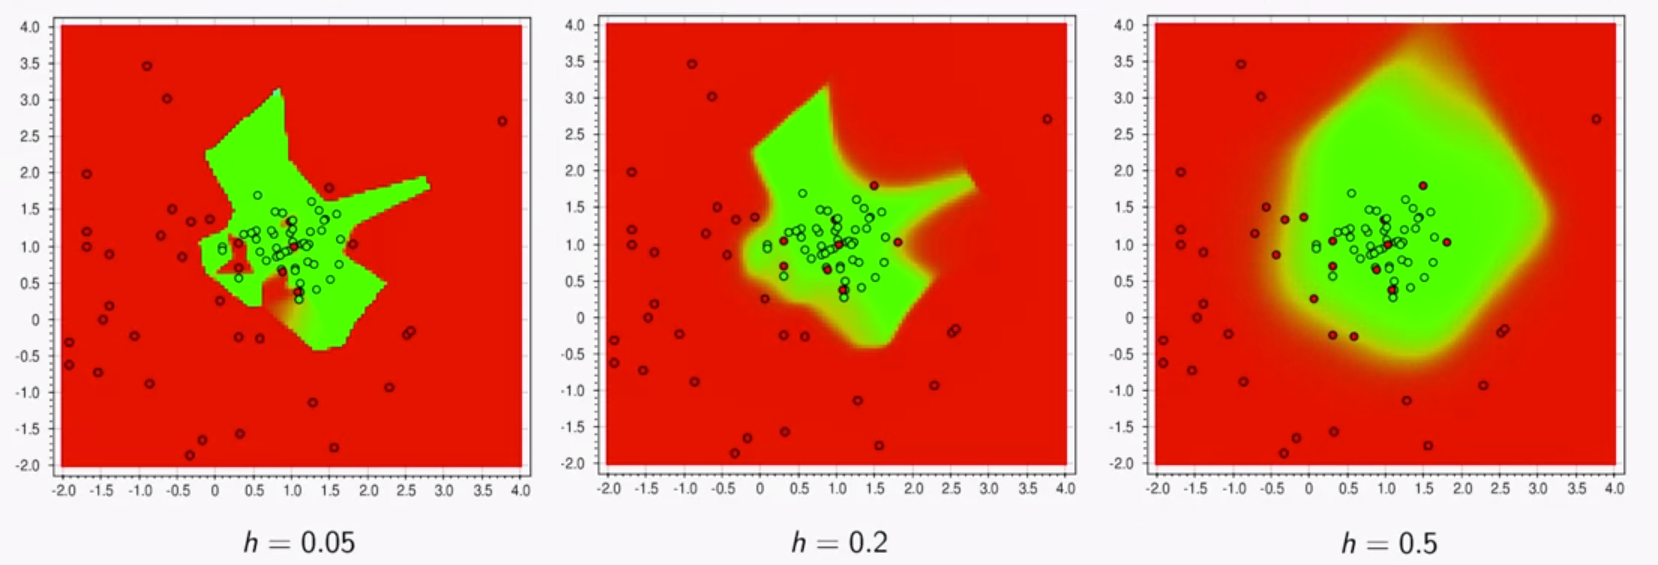
\includegraphics[scale=0.3]{images/4_3.png}
\end{center}

Серия графиков сейчас показывает, как меняется фактически граница между классами по мере увеличения ширины окна. Когда ширина окна была $0.1$, то фактически работал метод ближайшего соседа. Это слишком узкое окно. 

Далее, когда мы его потихоньку увеличиваем, граница между классами размазывается, становится более похожей на окружность. И на самом деле окружность --- это оптимальная граница между этими двумя классами. Мы их на самом деле так синтезировали, мы их так задумали. В данном случае облако точек зеленого цвета --- класс $(+1)$ --- распределен в сферической области.

Соответственно, алгоритм, который работал только по первому ближайшему соседу, очевидно, плохо восстанавливает эту сферическую область. С другой стороны, если сделать окно слишком широким, то в какой-то момент наш алгоритм классификации уже начинает вырождаться:

\begin{center}
    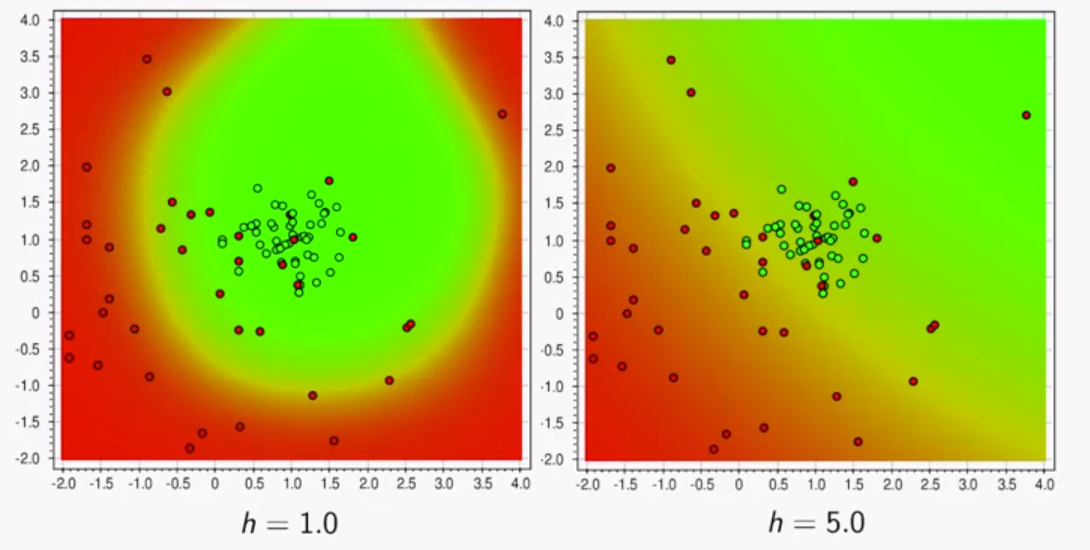
\includegraphics[scale=0.35]{images/4_4.png}
\end{center}

\newpage
\subsubsection{Метод потенциальных функций}

\begin{itemize}
\item[] $w(i, x) = \gamma^{(i)}K\Bigl(\frac{rho(x, x^{(i))}}{h^{(i)}}\Bigr)$

\item[] Более простая запись (без ранжирования объектов):

$$A(x;\ X^l) = arg\ \underset{y \in Y}{max}
\sum\limits_{i = 1}^l[y_i = y]\gamma_i K\Bigl(\frac{\rho(x, x^{(i)})}
{h_i}\Bigr),$$

где $\gamma_i$ --- веса объектов, $\gamma_i \geqslant 0$, $h_i > 0$.
\end{itemize}

Он очень \textit{похож} на метод парзеновского окна, но он меняет наш взгляд на то, что относительно чего расположено. Вот в методе парзеновского окна мы можем представить себя, стоящими в точке $x$ (это точка классифицируемого объекта), и мы смотрим на \textit{окрестность} этой точки (с учетом ширины окна) и подсчитываем число объектов, попавших в эту окрестность, а в итоге принимаем решение о классе.

Можно считать, что функция расстояния \textit{симметрична}, поэтому мы можем представить себя, стоящими по очереди в каждом обучающем объекте $x_i$, и думать, что каждый объект обучающей выборки распространяет вокруг себя \textit{потенциал} $gamma_i$ своего класса. Это прямая аналогия с \textbf{электростатикой}:

\begin{itemize}
\item[] $\gamma_i$ --- величина <<заряда>> в точке $x_i$;
\item[] $h_i$ --- <<радиус действия>> потенциала с центром в точке $x_i$;
\item[] $y_i$ --- знак <<заряда>> (в случае двух классов $Y = \{-1, +1\}$;
\item[] В электростатике $K(r) = \frac{1}{r}$ или $\frac{1}{r + a}$,\\
хотя в задачах классификации таких ограничений для $K$ нет, мы все еще можем подобрать любую функцию.
\end{itemize}

То есть можно представить представить себе, что точки --- это \textit{заряженные частицы} (положительные и отрицательные), то каждая точка \textit{распространяет} вокруг себя электрическое поле. И фактически знак этого поля в произвольной точке пространства $x$ как раз и покажет, \textit{к чему мы ближе}: к положительно заряженным объектам или к отрицательно заряженным объектам. 

Но этот метод хорош тем, что в нем теперь появляются параметры, и с каждым объектом обучающей выборки мы можем связать даже \textit{два числа}: $\gamma_i$ и $h_i$. Таким образом у нас получается классификатор, \textit{существенно обогащенный параметрами}. Теперь можно настраивать эти параметры по обучающей выборке. Собственно, \textit{алгоритм перестает быть ленивым}. Нам не только надо хранить обучающую выборку, но и настроить эти параметры. 
\\

\begin{center}
\line(1,0){400}
\end{center}


\textbf{Настройка параметров метода потенциальных функций}

Пусть имеем два класса: $Y = \{-1, +1\}$.

$$a(x) = arg\ \underset{y \in Y}{max}\text{Г}_y(x)
= sign(\text{Г}_{+1}(x) - \text{Г}_{-1}(x))
= sign\sum\limits_{i = 1}^l\gamma_i
\textcolor{red}{
	y_i K\Bigl(\frac{\rho(x, x^{(i)})}{h_i}\Bigr)
}.$$

Сравним с линейной моделью классификации:

$$a(x) = sign\sum\limits_{i = 1}^n\gamma_i \textcolor{red}{f_j(x)}.$$

\begin{itemize}
\item функции $\textcolor{red}{f_j(x)} = y_j K\bigl(\frac{1}{h_j}\rho(x, x_j)\bigr)$ --- признаки объекта $x$

\item $\gamma_j$ --- веса линейного классификатора

\item $n = l$ --- число признаков равно числу объектов обучения.
\end{itemize}

То есть на самом деле классификатор метода потенциальных функций --- \textit{это разновидность линейного классификатора}. 
\\

О линейных классификаторах мы будем говорить позднее, и изучим подробно методы, которыми можно настраивать веса в линейных классификаторах. Сейчас для нас принципиально важен факт, что здесь \textit{в качестве признаков} мы фактически \textit{используем функции близости} между классифицируемым объектом и объектом обучающей выборки. 

То есть каждый обучающий объект \textit{индуцирует} признак, и признаков здесь ровно столько, \textit{сколько объектов обучающей выборки}. Это глубинное сходство между метрическим классификатором (методом потенциальных функций) и линейным классификатором дает очень большую свободу при использовании линейных моделей классификации. 

Мы понимаем, что признаки --- это могут быть \textit{исходно имеющиеся} признаки, а можно в качестве признаков использовать \textit{близость до объектов} обучающей выборки. Это очень интересная возможность, которая в разных задачах может принести успех и повышение точности классификации.

\newpage
\section{Резюме}

\begin{itemize}
\item \textbf{Метрические классификаторы} --- одни из самых простых.\\
Качество классификации определяется качеством метрики.

\item \textbf{Что можно обучать:}
\begin{itemize}
\item число ближайших соседей $k$ или ширину окна $h$;
\item веса объектов;
\item набор эталонов (prototype selection);
\item метрику (distance learning, similarity learning);
\item веса признаков;
\item функцию ядра $K(r)$.
\end{itemize}
\end{itemize}

\end{document}
